\documentclass{standalone}
\usepackage{tikz}
\begin{document}
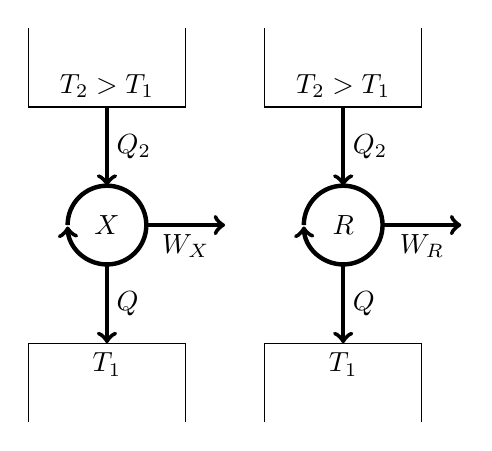
\begin{tikzpicture}[scale=2]
    \draw[-](-1,0)--(0,0);
    \draw[-](-1,0)--(-1,-0.5);
    \draw[-](0,0)--(0,-0.5);
    \node[below]at(-0.5,0){$T_1$};
   
    \draw[<-,ultra thick](-0.5,0)--(-0.5,0.5);
    \node[right]at(-0.5,0.25){$Q$};
    
    \draw[->,ultra thick](-0.75,0.75)arc(180:-178:0.25);
    \node[]at(-0.5,0.75){$X$};

    \draw[<-,ultra thick](-0.5,1)--(-0.5,1.5);
    \node[right]at(-0.5,1.25){$Q_2$};

    \draw[->,ultra thick](-0.25,0.75)--(0.25,0.75);
    \node[below]at(0,0.75){$W_X$};

    \draw[-](-1,1.5)--(0,1.5);
    \draw[-](-1,1.5)--(-1,2);
    \draw[-](0,1.5)--(0,2);
    \node[above]at(-0.5,1.5){$T_2>T_1$};



    \draw[-](0.5,0)--(1.5,0);
    \draw[-](0.5,0)--(0.5,-0.5);
    \draw[-](1.5,0)--(1.5,-0.5);
    \node[below]at(1,0){$T_1$};
   
    \draw[<-,ultra thick](1,0)--(1,0.5);
    \node[right]at(1,0.25){$Q$};
    
    \draw[->,ultra thick](0.75,0.75)arc(180:-178:0.25);
    \node[]at(1,0.75){$R$};

    \draw[<-,ultra thick](1,1)--(1,1.5);
    \node[right]at(1,1.25){$Q_2$};

    \draw[->,ultra thick](1.25,0.75)--(1.75,0.75);
    \node[below]at(1.5,0.75){$W_R$};

    \draw[-](0.5,1.5)--(1.5,1.5);
    \draw[-](0.5,1.5)--(0.5,2);
    \draw[-](1.5,1.5)--(1.5,2);
    \node[above]at(1,1.5){$T_2>T_1$};
\end{tikzpicture}
\end{document}